% Part V (label part:3). Merged 2026-10-03 (author approval); input in main.tex after part3/p3_05_coherence_optimum.
% Carried from two private device analyses (physics, method-step names, platform types, levers) under the public/proprietary ruling of
% 2026-10-03; every number below is either a published measured value (cited, DOI checked) or computed here from h, k_B and the
% stated gap, temperature and times (docs/book/figscripts/fig_p3_platforms.py and MANIFEST.md of the delivery). Nothing is fitted.
\chapter{Each platform on its own gauge: qubits}\label{ch:qplatforms}

\section*{The place}
IAM's Law (Chapter~\ref{ch:iams_law}) prices every irreversible record at $\kB T\ln2$ per bit at the nearest encoding surface, at that
surface's temperature. A qubit platform is fixed by two things: what its encoding surface is, and which temperature that surface
actually sees. The two differ from platform to platform, and so does the floor. This chapter takes the platforms one at a time:
superconducting transmons and fluxonium, trapped ions with laser and with electronic gates, neutral atoms, spin defects in diamond,
spin qubits in silicon, photons, and the proposed topological qubits. Each device is read against its own as-built state, on the
one gauge of Chapter~\ref{ch:onegauge}: its floor to the left, the device as built at 1, and the point where error correction fails
to the right. The platforms are not ranked against each other. Their errors come from different physics, and each field states its
thresholds in its own units \interp.

\section{Three marks on every qubit gauge}\label{sec:qp_marks}
\paragraph{As built.} The reading is the gate error in nats, $\varepsilon=-\ln(1-p_{2Q})$ (Eq.~\eqref{eq:Agate}), of the device as
it was built and benchmarked. It is the denominator of the gauge, so the device reads $A=1$.

\paragraph{Full surface.} On the right is the error at which the device stops being able to protect a record by error correction.
For the surface code it is about $10^{-2}$ per operation~\cite{Fowler2012}; on the gauge it sits at $10^{-2}/\varepsilon$ \calc. A
platform that uses a different code, or a measurement-based scheme, carries the threshold of that scheme instead. For the colour code, which reconfigurable neutral-atom arrays with arbitrary connectivity have run on up to 40 logical
qubits~\cite{Bluvstein2024} \observed, the storage threshold of the triangular colour code under circuit-level depolarising noise has been
estimated at 0.2\,\%~\cite{Chamberland2020NJP} \observed, so its right-hand mark sits five times further left than the surface code's
\calc. A threshold belongs to a code, a decoder and a noise model together \interp.

\paragraph{The floor from $\kB T$.} On the left is the lowest error the record can hold before thermal kicks win. For a record held
in a two-level system with gap $E=hf$, in contact with a bath at temperature $T$, detailed balance fixes the ratio of the upward and
downward rates, $\Gamma_\uparrow/\Gamma_\downarrow=e^{-E/\kB T}$. With $\Gamma_1=\Gamma_\uparrow+\Gamma_\downarrow=1/T_1$ the equilibrium
occupation of the wrong level is
\begin{equation}
 p_{\rm eq}=\frac{1}{1+e^{M}},\qquad M=\frac{E}{\kB T},
 \label{eq:qp_peq}
\end{equation}
and a record prepared in the right level and held for a time $t\ll T_1$ is kicked out of it with probability
\begin{equation}
 p_{\rm th}(t)=\Gamma_\uparrow t=p_{\rm eq}\,\frac{t}{T_1}
 \label{eq:qp_pth}
\end{equation}
\derived\ (detailed balance). $M$ is the Mahaffey number of the record (Eq.~\eqref{eq:law_mahaffey}): the energy holding it against
the thermal quantum of the bath it touches. Equation~\eqref{eq:qp_peq} has the form of the cell's copy-error floor
$\varepsilon_0=1/(1+e^{E_{\rm hold}/\kB T})$ (Chapter~\ref{ch:onegauge}); the cell holds its bit with chemical energy, the qubit with
the gap of its encoding degree of freedom. For a bosonic record (a motional mode, a radiation mode) the occupation is
$\bar n=1/(e^{M}-1)$. The floor of a record held for long times is $p_{\rm eq}$; the floor of one gate of duration $t_g$ is
$p_{\rm th}(t_g)$. Every thermal kick that is later undone by correction, or that is lost, is an erasure, and IAM's Law prices it at no
less than $\kB T\ln2$ at the temperature of the bath that delivered it \interp. This thermal floor is the left-hand mark of every qubit
gauge in this book: it needs no fitted constant, only the gap, the temperature the record sees, the gate time and $T_1$, all of which a
laboratory already measures.

\paragraph{A worked reading.} For a transmon at $f=5$~GHz whose own effective temperature is 35~mK~\cite{Jin2015}, $M=6.86$ and
$p_{\rm eq}=1.05\times10^{-3}$. With the mean $T_1=68~\mu$s of the 105-qubit processor of Ref.~\cite{GoogleWillow2025} and an
illustrative gate time $t_g=40$~ns, $p_{\rm th}(t_g)=6.2\times10^{-7}$ \calc. A two-qubit error near $10^{-3}$ therefore sits about
1,600 times above its thermal floor, and on its own gauge the floor sits near $6\times10^{-4}$. At the 15~mK of the mixing chamber the
same gap would give $M=16.0$ and $p_{\rm eq}=1.1\times10^{-7}$ \calc: the qubit is hotter than its refrigerator, and the floor is set by
the qubit's temperature, not the refrigerator's.

\section{Which temperature each record sees}\label{sec:qp_which}
Table~\ref{tab:qp_which} and Figure~\ref{fig:qp_floors} collect, for each platform, the degree of freedom that holds the record, its gap,
the temperature that degree of freedom actually couples to, and the resulting $M$ and thermal occupation. The table is the first step of
every reading in this chapter: a floor computed at the wrong temperature is a floor of a different device.

\begin{table}[htbp]\centering\small
\caption{The record, its gap and the temperature it sees, platform by platform. $M=hf/\kB T$; occupation from Eq.~\eqref{eq:qp_peq}
(two-level records) or $\bar n=1/(e^M-1)$ (modes). Values \calc\ from the stated gap and temperature; the temperatures quoted from
experiments are \observed\ as cited.}\label{tab:qp_which}
\begin{tabularx}{\linewidth}{@{}>{\raggedright\arraybackslash}p{0.15\linewidth}>{\raggedright\arraybackslash}X>{\raggedright\arraybackslash}p{0.21\linewidth}>{\raggedright\arraybackslash}p{0.12\linewidth}>{\raggedright\arraybackslash}p{0.15\linewidth}@{}}\toprule
platform & record and gap & temperature it sees & $M$ & occupation \\\midrule
transmon & charge--phase states of the junction circuit, 5~GHz & the qubit itself, 35~mK~\cite{Jin2015} (refrigerator 15~mK) & 6.86 (16.0) & $1.1\times10^{-3}$ ($1.1\times10^{-7}$)\\
fluxonium & flux states of a superinductor loop, 0.2--1~GHz & as transmon, 20~mK & 0.48--2.4 & 0.38--0.083\\
ion, spin & hyperfine levels, 3.2~GHz ($^{43}$Ca$^+$), 8.0 ($^{137}$Ba$^+$), 12.6 ($^{171}$Yb$^+$) & none: the spin is isolated, not thermalised & ($5\times10^{-4}$--$2\times10^{-3}$ at 300~K) & set by optical pumping, not by $T$\\
ion, motion (gate bus) & axial mode, 1--2~MHz & motional temperature; Doppler limit 0.47~mK for Yb$^+$ & 0.10--0.20 & $\bar n=9.3$--4.4\\
neutral atom & Rydberg transitions, 10--100~GHz & the radiation field, 300~K (4~K in a cryogenic array) & 0.0016--0.016 (0.12--1.2) & $\bar n=620$--62 (7.8--0.43)\\
NV centre & electron-spin triplet, $D=2.87$~GHz & the diamond lattice, 300~K (4~K) & $4.6\times10^{-4}$ (0.034) & sublevels equal to $10^{-3}$\\
silicon spin & Zeeman levels, 3.5--15~GHz & electrons near 0.1~K; ``hot'' operation 1.5~K~\cite{Yang2020hot} & 7.2 (15~GHz, 0.1~K); 0.11 (3.5~GHz, 1.5~K) & $7.5\times10^{-4}$; 0.47\\
photon & one optical photon, 1550~nm (193~THz) & the waveguide, 300~K; detectors a few kelvin & 30.9 & $3.7\times10^{-14}$\\\bottomrule
\end{tabularx}
\end{table}

\begin{figure}[htbp]\centering
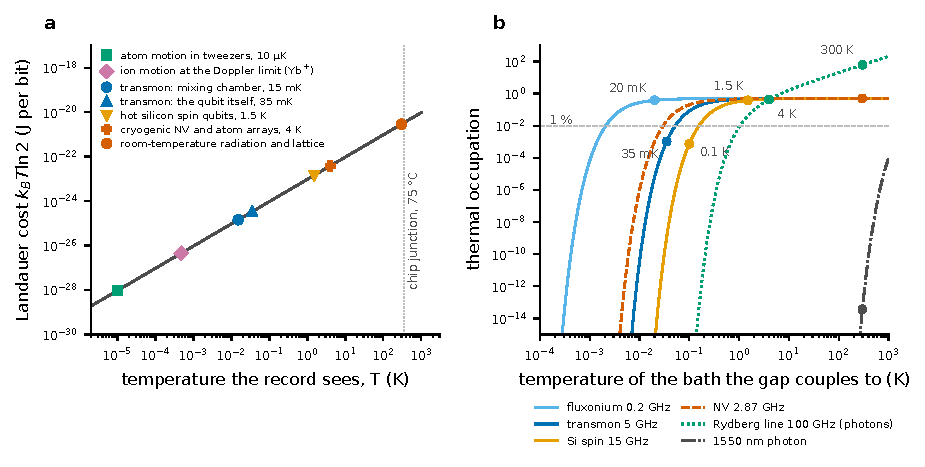
\includegraphics[width=\textwidth]{figures/part3/fig_p3_platform_floors.pdf}
\caption{(a) The Landauer cost $\kB T\ln2$ per bit at the temperature each record actually sees: from $10^{-28}$~J for atoms moving at
10~$\mu$K to $3\times10^{-21}$~J for anything in contact with room-temperature radiation or lattice; the chip junction at 75\,$^\circ$C is
marked for comparison. (b) Thermal occupation of each platform's encoding gap against the temperature of the bath it couples to:
two-level records (solid, dashed) and photons per mode (dotted, dash-dotted); dots at the operating points of Table~\ref{tab:qp_which}.
Dashed grey: 1\,\%. \calc}\label{fig:qp_floors}
\end{figure}

Three lessons follow directly from the table \interp. First, for every platform except the photon, some degree of freedom in the gate
sits near or below $M\approx1$: the transmon's own electrodes and quasiparticles, the ion's motion, the Rydberg atom's radiation field,
the NV lattice, the hot silicon spin. The platforms differ in which degree of freedom that is and in how short the gate is compared with
its relaxation. Second, a large $M$ for the record does not protect a gate that passes through a small-$M$ degree of freedom: the ion's
spin is perfectly isolated, but its gate runs through the motion. Third, the photon has $M=30.9$ at room temperature, so thermal kicks
play no part in its error; what erases its record is loss.

\section{Superconducting transmons}\label{sec:qp_transmon}
\paragraph{The surface and its temperature.} The record is the state of the junction circuit (Chapter~\ref{ch:scprimer}); the surfaces
that write on it are the amorphous oxides at the metal--air, metal--substrate and substrate--air interfaces and on the junction leads,
where most two-level-system (TLS) loss sits~\cite{Wang2015TLS,Lisenfeld2019,Lisenfeld2025}, and the quasiparticle density of the
electrodes (Chapter~\ref{ch:xqp}). The junction itself is Al/AlO$_x$/Al whatever the base metal of the pads and wiring. The temperature
that matters is the qubit's own effective temperature, which in a careful 3D-transmon measurement followed the refrigerator from 150
down to 35~mK and then saturated, with a residual excited-state occupation of 0.1\,\%~\cite{Jin2015} \observed.

\paragraph{Where the dissipation goes.} The gate error splits into a coherence part $p_{\rm coh}\approx t_g/T_1+t_g/T_\phi$ up to
state-averaging factors~\cite{Abad2022}, the thermal-kick part of Eq.~\eqref{eq:qp_pth}, a material part from the TLS bath, and control
and crosstalk (Eq.~\eqref{eq:pdecomp}). Only the first two follow from standard theory \derived; the split of the remainder between
material and control is a model (Chapter~\ref{ch:walls}) \conjecture. The worked reading of Section~\ref{sec:qp_marks} shows that the
thermal-kick part is three orders of magnitude below a present two-qubit error: of the channels that write on a transmon, the thermal
one is the furthest above its floor in the wrong direction, that is, the least important \calc. The 105-qubit processor of
Ref.~\cite{GoogleWillow2025} reports a mean $T_1=68~\mu$s and $T_{2,\rm CPMG}=89~\mu$s \observed.

\paragraph{Levers.} Four engineering levers act on a superconducting qubit: eliminating the interface, geometric decoupling via
participation ratio engineering, oxide phase reduction via material selection, and operating frequency engineering. Participation ratio
engineering is a geometric technique that reduces the fraction of the qubit's electric field energy stored in the lossy oxide layer,
without changing the oxide material itself; for a transmon the interface cannot be eliminated, because the junction is the qubit. A tantalum base layer lowers the surface-oxide
loss and raised $T_1$ to 0.3--0.5~ms~\cite{Place2021,Wang2022Ta}; its native oxide is amorphous Ta$_2$O$_5$ with suboxides near the
metal~\cite{Crowley2023} \observed; the junction barrier keeps its own Al/AlO$_x$ oxide in every case. The levers do not all act on the
same mark of the gauge. The key distinction is between levers that move the gate error and levers that move the ceiling. A substrate
change does not improve today's gate error at all; it raises the coherence a later device on that material can reach. It does not fix
today; it buys runway for tomorrow \interp.
Lowering the qubit's effective temperature moves the thermal floor; shortening the gate moves both the coherence part and the
thermal-kick part.
The refrigerator does not set that temperature by itself: the dilution refrigerator of Ref.~\cite{Krinner2019} has its mixing chamber
at 6~mK, while a qubit's own temperature saturated at 35~mK as the refrigerator went lower~\cite{Jin2015} \observed, so this lever acts
through the qubit's thermalisation and filtering more than through the base temperature \interp. A further lever is the gate itself:
redesigning the two-qubit gate changes which channel binds without changing the material \interp. The geometric lever has been measured
directly. With a clean electromagnetic environment and the non-equilibrium quasiparticle density suppressed, the relaxation rates of 3D
transmons were found approximately proportional to their surface participation ratios~\cite{Wang2015TLS} \observed: a device carries two
floors, the dielectric one that geometry and material move, and the quasiparticle one, which shielding, filtering and gap engineering
move (Chapter~\ref{ch:xqp}) \interp. The material and geometric levers have been combined: a tantalum-based platform on annealed
sapphire, with device geometry optimised for coherence, gave on-chip quantum memories with energy relaxation times of
1.0--1.4~ms~\cite{Ganjam2024} \observed.

\paragraph{What a laboratory learns.} From $T_1$, $T_\phi$, $t_g$, the effective temperature and the isolated two-qubit error measured on
one device, the reading gives the share of the error that coherence forces, the share thermal kicks force, and what is left for the
material and the control. A material change then shows up as a change of the remainder at fixed coherence, and a change of coupler
graph as a change of the simultaneous error at fixed isolated error.

\paragraph{What a referee would confirm.} The excited-state occupation against refrigerator temperature on the same device (the
protocol of Ref.~\cite{Jin2015}); isolated and simultaneous two-qubit errors on one stated benchmark~\cite{Proctor2022}, since a
layered-circuit error per gate includes crosstalk and idling and is a different quantity~\cite{McKay2023}; and TLS spectroscopy that
locates the fluctuators~\cite{Lisenfeld2019,Lisenfeld2025}. The coherence-optimum test of Chapter~\ref{ch:walls} needs all of these on
one material and one coupler topology \openprob.

\section{Fluxonium}\label{sec:qp_fluxonium}
\paragraph{The surface and its temperature.} Fluxonium shunts a small junction with a large inductance and runs at a few hundred
megahertz to about a gigahertz. The lower frequency lowers the coupling to the same lossy surfaces per cycle: a fluxonium has reached a
Ramsey coherence time $T_2^*=1.48\pm0.13$~ms with single-qubit gate fidelity above 0.9999~\cite{Somoroff2023}, and a fluxonium pair coupled
through a transmon has reached a mean CZ fidelity of $99.922\pm0.009$\,\%~\cite{Ding2023} \observed, that is $\varepsilon=7.8\times10^{-4}$,
with the surface-code threshold at 12.9 on its own gauge \calc.

\paragraph{The frequency lever has a thermal price.} The same low frequency lowers $M$. At 20~mK a 1~GHz fluxonium has $M=2.4$ and an
equilibrium occupation of 8\,\%; at 0.2~GHz, $M=0.48$ and 38\,\% \calc. The held record therefore needs active reset or heralded
preparation, while the per-gate thermal floor, Eq.~\eqref{eq:qp_pth}, stays small because $T_1$ is long. The operating-frequency lever
moves the coherence part and the thermal floor in opposite directions \derived.

\paragraph{What a laboratory learns; what a referee would confirm.} The trade is measurable on one device: initial-state occupation and
$T_1$ at two operating frequencies, at one refrigerator temperature.

\section{Trapped ions with laser-driven gates}\label{sec:qp_ionlaser}
\paragraph{The surface and its temperature.} The record is a hyperfine level pair of an ion in vacuum, with no solid surface and no oxide
in contact with it. Its spin is not thermalised by anything: at 300~K its $M$ is $10^{-3}$, and its state is set by optical pumping, not by
temperature (Table~\ref{tab:qp_which}). The two-qubit gate, however, runs through the shared motion of the ions, and that motion has a
temperature: the cooling limit (the Doppler limit of Yb$^+$ is 0.47~mK) plus the heating driven by electric-field noise from the trap
electrodes~\cite{Brownnutt2015}. At the Doppler limit a 1~MHz mode holds $\bar n=9.3$ quanta \calc. An ion has no superconducting gap and no Cooper pairs, so the quasiparticle channel of Chapter~\ref{ch:xqp} has no counterpart in it,
nor in a neutral atom or in a photon in flight; that channel returns wherever a superconductor enters the record, as in the proximitised
wire of a topological qubit (Section~\ref{sec:qp_topo}) or the superconducting detectors of a photonic computer \interp.

\paragraph{Where the dissipation goes.} Three channels: laser noise, motional heating and control. Two of them
change in opposite directions with the drive, which gives the drive optimum of Eq.~\eqref{eq:walls_mhi} (Chapter~\ref{ch:walls}); the point
where the falling laser-noise part meets the rising heating part is the drive optimum of the ion gate \conjecture\ (form).
The electrodes have a thermal floor of their own: Johnson--Nyquist noise, whose spectral density scales with the electrode temperature
times its resistance~\cite{Brownnutt2015} \derived. Measured heating lies far above it, and in surface traps cooled to 6~K the heating
rates fell by seven orders of magnitude~\cite{Labaziewicz2008} \observed: of the ion's channels, motional heating is the one furthest above
its thermal floor, and the one that cooling the electrodes moves. Spontaneous Raman scattering from the gate beams sets a further,
non-thermal floor for laser gates~\cite{Ozeri2007} \observed. Background heating rates of $29\pm4$ quanta/s for the centre-of-mass mode and
$3.0\pm0.5$ quanta/s for the stretch mode were measured for a $^{138}$Ba$^+$--$^{171}$Yb$^+$ crystal in an X-junction surface-electrode
trap~\cite{Burton2023} \observed. Published two-qubit errors: Helios ($^{137}$Ba$^+$) $7.9(2)\times10^{-4}$ averaged over all operational
zones~\cite{Ransford2025}, H2 ($^{171}$Yb$^+$) $1.57\times10^{-3}$~\cite{DeCross2025}, Forte ($^{171}$Yb$^+$) $4.64\times10^{-3}$ median by direct
randomized benchmarking~\cite{Chen2024Forte} \observed. Each is read on its own gauge, against its own as-built reference. The record itself is long-lived. For a $^{171}$Yb$^+$ hyperfine qubit, with a co-trapped $^{138}$Ba$^+$ ion laser-cooled throughout,
process tomography gave $T_1=12000\pm2200$~s and $T_2=4200\pm580$~s, and a coherence time of about 5500~s was reached after the
remaining magnetic-field fluctuations, the frequency instability of the microwave reference oscillator and its leakage were
suppressed~\cite{WangYb2021} \observed. On the held record the leading channels are therefore magnetic-field and reference noise, and
$T_1$ is not what limits an ion's gates \interp. How the error-correction overhead of an ion processor follows from these times, rather
than from its gate channels, has not been worked out on its own gauge \openprob.

\paragraph{Levers.} Sympathetic cooling with a co-trapped species lowers the motional temperature during an algorithm and moves the drive
optimum outward \interp; cryogenic electrodes and surface treatment lower the heating; a different gate class removes the laser channel
(Section~\ref{sec:qp_ionelec}). The physics of sympathetic cooling is the separation of the two species. When the cooling transitions of the coolant and the qubit
ion are far apart (more than 30~nm for $^{9}$Be$^+$ and $^{24}$Mg$^+$), laser light on one has negligible effect on the other, so the
motion can be re-initialised without touching the stored information, the coolant taking up the motional energy through
the modes the two ions share~\cite{Barrett2003} \observed. Even isotopes can serve: a $^{43}$Ca$^+$ memory qubit sympathetically cooled by a
$^{40}$Ca$^+$ coolant near the ground state of both axial modes lost 3.3\,\% of its coherence per cooling cycle, against a natural limit
of order $10^{-4}$ per cycle~\cite{Home2009} \observed.

\paragraph{What a laboratory learns; what a referee would confirm.} Per-mode heating rates and $\bar n$ at the start of the gate, the
scattering rate per gate and the laser phase-noise spectrum split the error into its parts. The drive optimum is located by measuring the
two-qubit error against drive power at fixed heating; repeating that measurement with and without sympathetic cooling shows how far the
cooling moves the optimum.

\section{Trapped ions with electronically driven gates}\label{sec:qp_ionelec}
The electronic gate applies a spin-dependent force from electrode currents and microwaves rather than from lasers. In the ``smooth gate''
the residual spin--motion entanglement is eliminated adiabatically by ramping the gate detuning: two-qubit gates with an estimated error
of $8.4(7)\times10^{-5}$ without ground-state cooling, and an error that remains $\lesssim5\times10^{-4}$ up to a mean phonon occupation of
$\bar n=9.4(3)$ on the gate mode~\cite{Hughes2025} \observed. In the language of Table~\ref{tab:qp_which}, the gate has been made
insensitive to the one degree of freedom with $M<1$: the motional thermal floor has been engineered out of the gate rather than cooled away,
and the laser-scattering floor is absent because there is no laser in the gate \interp. What remains is the noise of the control chain and
of the electrodes. On its own gauge the surface-code threshold sits at 120 \calc.

\section{Neutral atoms}\label{sec:qp_atoms}
\paragraph{The surface and its temperature.} The record is a pair of long-lived ground levels of an atom held in an optical tweezer; the
gate excites the atoms briefly to Rydberg states whose blockade makes the interaction. Two temperatures matter, and they are four orders of
magnitude apart \interp. The atoms' motion, near 10~$\mu$K, sets Doppler and position errors. The radiation field around the atoms, at
room temperature in most arrays, drives transitions out of the Rydberg state: Rydberg transitions at 10--100~GHz see $\bar n=620$--62
thermal photons per mode at 300~K, \calc; blackbody-induced transition rates and effective lifetimes of alkali Rydberg states have been calculated
at 77, 300 and 600~K~\cite{Beterov2009}. In a 4~K environment the same modes hold 7.8--0.43 photons \calc; tweezer arrays have been operated at cryogenic temperature
with single-atom trapping lifetimes of 6000~s~\cite{Schymik2021} \observed.

\paragraph{Where the dissipation goes, and a drive optimum.} A stronger Rydberg drive $\Omega$ shortens the time spent in the Rydberg state,
so the decay part falls as $a/\Omega$; it raises leakage out of the blockade and scattering from the intermediate state, which grow roughly
as $b\Omega^2$. Their sum,
\begin{equation}
 p(\Omega)=\frac{a}{\Omega}+b\,\Omega^2+p_{\rm ctrl},\qquad \Omega^*=\Bigl(\frac{a}{2b}\Bigr)^{1/3},\qquad p(\Omega^*)-p_{\rm ctrl}=\frac{3a}{2\Omega^*},
 \label{eq:qp_rydberg}
\end{equation}
has a minimum at $\Omega^*$ \derived\ (within the model). The form is a \conjecture; $a$ and
$b$ are properties of each apparatus and have to be measured. Two-qubit entangling gates with 99.5\,\% fidelity have been run on up to 60
atoms in parallel~\cite{Evered2023} \observed, that is $\varepsilon=5.0\times10^{-3}$, with the surface-code threshold at 2.0 on its own
gauge \calc.

\paragraph{Levers.} Cooling the atoms' motion is already done; cooling the radiation environment lowers the blackbody part of the Rydberg
decay; the drive sits at its own optimum. The statement that temperature reduction will not improve Rydberg gate fidelity holds for the
atoms' motion and for the ground-state record, and not for the radiation field seen by the Rydberg state \interp.

\paragraph{What a laboratory learns; what a referee would confirm.} The Rydberg lifetime measured in place, at the environment temperature
of the experiment, and the gate error against drive strength on the same apparatus, give $a$, $b$ and the share of the error that the
radiation field delivers.

\section{Spin defects in diamond}\label{sec:qp_nv}
\paragraph{The surface and its temperature.} The NV centre's record is its electron-spin triplet, split by $D=2.87$~GHz at zero field,
with nuclear spins of the lattice as memory. At room temperature $M=4.6\times10^{-4}$: the three sublevels are equally occupied to one part in
a thousand, and the state is prepared by optical pumping \calc. The temperature that writes on the record is the lattice's: above room
temperature a two-phonon Raman process dominates the longitudinal relaxation, below it an Orbach-type process with activation energy
$73(4)$~meV, and at the lowest temperatures sample-dependent cross-relaxation leaves $T_1$ between milliseconds and minutes~\cite{Jarmola2012}
\observed. The thermal floor per gate, Eq.~\eqref{eq:qp_pth}, therefore carries a temperature dependence that is a power law over one window
and activated over another; a single exponent describes it only locally (Chapter~\ref{ch:thermaln}).

\paragraph{The published gate, and the levers.} An electron--nuclear two-qubit gate set characterised by gate-set tomography has reached a
two-qubit gate fidelity of $99.93(5)$\,\%~\cite{Bartling2025} \observed, $\varepsilon=7.0\times10^{-4}$, with the surface-code threshold at 14.4
on its own gauge \calc. The levers are cooling (which freezes out the Raman and Orbach channels), isotopic purification of the lattice (fewer
nuclear spins in the bath), and decoupling sequences that keep the gate insensitive to the remaining bath.

\paragraph{What a laboratory learns; what a referee would confirm.} $T_1$ against temperature on the device separates the three channels and
shows which one is closest to its floor at the operating temperature; the gate error at two temperatures tests whether the gate is limited
by the lattice at all.

\section{Spin qubits in silicon}\label{sec:qp_si}
\paragraph{The surface and its temperature.} The record is the spin of an electron in a gate-defined quantum dot, with a Zeeman gap of a few
to about twenty gigahertz. The temperature that writes on it is the electrons' and the lattice's, near 0.1~K in a dilution refrigerator.
Silicon spin qubits have also been run ``hot'': a two-qubit unit cell at about 1.5~K, at a control frequency of 3.5~GHz where, in the paper's
words, the qubit energy is well below the thermal energy~\cite{Yang2020hot}, and universal two-qubit logic above one kelvin~\cite{Petit2020hot}
\observed. At 3.5~GHz and 1.5~K, $M=0.11$ and $p_{\rm eq}=0.47$ \calc: the held record is close to random, yet the gates work.

\paragraph{The held record and the gate are different floors.} The hot spin qubit is the cleanest case of the distinction in
Section~\ref{sec:qp_marks}. Its equilibrium floor is high, but initialisation is done by tunnelling rather than by waiting for equilibrium,
and the gate is short compared with $T_1$, so the per-gate thermal floor $p_{\rm eq}t_g/T_1$ stays small \derived. Two-qubit fidelities: all
gate fidelities above 99.5\,\% by gate-set tomography~\cite{Xue2022}, a two-qubit gate fidelity of 99.5\,\%~\cite{Noiri2022}, and single- and
two-qubit control fidelities exceeding 99\,\%~\cite{Mills2022} \observed; at 99.5\,\%, $\varepsilon=5.0\times10^{-3}$ and the surface-code
threshold sits at 2.0 \calc.

\paragraph{Levers; what a laboratory learns; what a referee would confirm.} The magnetic field raises $M$ in proportion; isotopic enrichment
removes the hyperfine bath of $^{29}$Si; the operating temperature trades cooling power against the held-record floor. $T_1$ and the
initial-state occupation against temperature, on one device, give both floors and say how far the operating temperature can rise for a
target error.

\section{Photons}\label{sec:qp_photon}
At 1550~nm and room temperature an optical photon has $M=30.9$ and a thermal occupation of $3.7\times10^{-14}$ \calc. Thermal kicks play no
part in a photonic record. What erases it is loss: a photon absorbed or scattered out of its mode is a record written into the environment.
The noise mechanism is fabrication loss: waveguide scattering, photon source indistinguishability, and detector efficiency. The record that is finally kept is written at the detector, and the
detectors are superconducting and cold; on IAM's reading the encoding surface of a photonic computation is the detector, at the detector's
temperature \interp. A manufacturable silicon-photonic platform has reported dual-rail qubits with $99.98\pm0.01$\,\% state preparation and
measurement fidelity, Hong--Ou--Mandel visibility $99.50\pm0.25$\,\% between independent sources, two-qubit fusion with $99.22\pm0.12$\,\%
fidelity and a chip-to-chip interconnect with $99.72\pm0.04$\,\% fidelity, conditional on photon detection and not accounting for
loss~\cite{PsiQuantum2025} \observed. Fusion is a measurement, not a gate, and the threshold of a fusion-based scheme is stated jointly in
loss and fusion error; the right-hand mark of the photonic gauge is scheme-specific \openprob.

\section{Topological qubits}\label{sec:qp_topo}
The proposed topological qubit stores its record in the shared fermion parity of Majorana zero modes at the ends of a proximitised
semiconductor nanowire. The thermal kick on such a record is quasiparticle poisoning, which flips the parity; its source is the same
non-equilibrium quasiparticle background as in Chapter~\ref{ch:xqp} \interp. A single-shot interferometric parity measurement in
InAs--Al devices has been reported, with a parity dwell time longer than 1~ms at in-plane fields of about 2~T~\cite{Aghaee2025}
\observed. The paper states that these measurements do not, by themselves, determine whether the low-energy states detected are topological,
and the journal's editorial team noted that the results do not represent evidence for Majorana zero modes~\cite{Aghaee2025}. The field reads such results with care for a reason: a 2018 report of quantized Majorana conductance in hybrid nanowires was retracted
in 2021 after a re-analysis of its raw data and a re-calibration, its authors writing that they could no longer claim the
observation~\cite{Zhang2021Retraction} \observed. In a tetron device with two parallel nanowires, single-shot parity measurements of two
loops designed as Pauli-$X$ and $Z$ measurements gave parity-switching times of $14.5\pm0.3~\mu$s and $12.4\pm0.4$~ms and estimated
assignment errors of 16\,\% and 0.5\,\%~\cite{Tetron2026} \observed. These are single-qubit measurement results, not entangling gates
\interp. No two-qubit
gate error has been published, so no device of this class can yet be placed on its gauge \openprob. Its first published two-qubit error,
read with the gate time, $T_1$ and the parity lifetime of the same device, will place it on the same three marks as every other platform.

\section{The method steps and what each does}\label{sec:qp_steps}
The readings above use the same short sequence of steps on every platform. Table~\ref{tab:qp_steps} names each step, says what it does and
why it is there.

\begin{table}[htbp]\centering\small
\caption{The method steps of the device gauges, for qubits (this chapter) and chips (Chapter~\ref{ch:chipgen}).}\label{tab:qp_steps}
\begin{tabularx}{\linewidth}{@{}>{\raggedright\arraybackslash}p{0.22\linewidth}>{\raggedright\arraybackslash}X>{\raggedright\arraybackslash}p{0.30\linewidth}@{}}\toprule
step & what it does & why \\\midrule
gate error in nats & re-expresses $p_{2Q}$ as $\varepsilon=-\ln(1-p)$, information lost per gate & the gauge works in information; $\varepsilon\approx p$ below $10^{-2}$ \\
which temperature & names the degree of freedom that holds the record and the bath it touches; computes $M$ and the occupation & a floor at the wrong temperature belongs to a different device \\
the one gauge & places the floor, the device as built ($=1$) and the full-surface mark on one axis & reads each device against itself, never against another \\
error decomposition & splits the error into coherence, thermal-kick, material and control parts (superconductors) or laser, motional and control parts (ions) & shows where the dissipation goes and which channel is closest to its floor \\
coherence-optimum check & asks whether more $T_1$ on unchanged material still lowers the error (Chapter~\ref{ch:walls}) & separates a material limit from a control limit \\
drive-optimum check & locates the drive at which a falling and a rising part of the error are equal (Eqs.~\eqref{eq:walls_mhi}, \eqref{eq:qp_rydberg}) & tells whether more drive helps or hurts \\
generation comparison & compares a device with its predecessor on one stated benchmark & a rise is a signal only on matched statistics~\cite{Proctor2022,McKay2023} \\
lever map & sorts each engineering change by the mark it moves: the as-built reading or a floor & separates changes that improve today from changes that make room \\
connectivity reading & carries an isolated two-qubit error to a gate inside a full circuit (Chapter~\ref{ch:walls}) & published errors are measured with neighbours idle \\
step-series end & a constant fractional improvement per generation crosses the floor after a finite number of generations, so it must slow before it & the floor cannot be crossed (Chapter~\ref{ch:cmos}) \\\bottomrule
\end{tabularx}
\end{table}

\section{What the readings can do for each field}\label{sec:qp_use}
For a laboratory the readings answer three questions from numbers the laboratory already measures \interp: where the dissipation goes (the
decomposition), which loss channel is closest to its own floor (each channel against the floor of the bath that drives it), and which lever
moves which mark (the lever map). For a referee they say which numbers must come from the same device and the same benchmark before any
statement about a floor can be checked: the gate error, the gate time, $T_1$ and $T_\phi$ or their equivalents, and the temperature of the
degree of freedom the gate passes through. The readings do not rank platforms and do not forecast them.

\section{Status}
Derived: the thermal floor of a held record, $p_{\rm eq}=1/(1+e^M)$, and of one gate, $p_{\rm eq}t_g/T_1$, from detailed balance; the drive
optimum of a Rydberg gate within its two-term model \derived. Calculated from stated gaps, temperatures and times: Table~\ref{tab:qp_which},
Figure~\ref{fig:qp_floors} and the threshold marks \calc. Published values as cited \observed. The forms of the drive optima are
\conjecture. The thermal floor derived here is the left-hand mark of the qubit gauge throughout the book, in the one-gauge chapter as here.
Open, and ready for any laboratory that measures the four inputs on one device: how close each loss channel comes to the floor of the bath
that drives it; the right-hand mark for fusion-based photonic schemes; a first gate for topological qubits \openprob.
